\chapter{กล้องจุลทรรศน์และเทคนิคการย้อมสีจุลินทรีย์}
\label{chap:ch04}

\section*{แผนบริหารการสอนประจำบทที่ 4}
\addcontentsline{toc}{section}{แผนบริหารการสอนประจำบทที่ 4}

\noindent\textbf{. หัวข้อเนื้อหาประจำบท}

\begin{enumerate}
    \item 4.1 หลักการเตรียมสเมียร์และการตรึงเซลล์ด้วยความร้อน (Heat Fixation)
    \item 4.2 ทฤษฎีประจุของสีย้อมชีวภาพ (Basic \& Acidic Dyes)
    \item 4.3 กลไกการย้อมสีแกรมตามโครงสร้างผนังเซลล์ Peptidoglycan (Gram+ vs Gram-)
    \item 4.4 ขั้นตอนการย้อมสีแกรม 4 สเต็ป (Crystal Violet, Iodine, 95\% Alcohol, Safranin)
    \item 4.5 ปัจจัยที่มีผลต่อความคลาดเคลื่อนในการย้อมสีแกรม (อายุของเชื้อและการล้างสีเกินขนาด)
\end{enumerate}

\noindent\textbf{. วัตถุประสงค์เชิงพฤติกรรม}

\begin{enumerate}
    \item เมื่อนักศึกษาได้เรียนรู้และปฏิบัติการทดลองประจำบทนี้แล้ว จะต้องมีความรู้ความสามารถดังต่อไปนี้:
    \item อธิบายความแตกต่างทางโครงสร้างผนังเซลล์ของแบคทีเรียแกรมบวกและแกรมลบได้
    \item เตรียมสเมียร์ ตรึงเชื้อ และย้อมสีแกรม 4 ขั้นตอนได้อย่างถูกต้องและแม่นยำ
    \item ส่องตรวจและจำแนกแบคทีเรียแกรมบวก (สีม่วง) และแกรมลบ (สีชมพูแดง) ใต้กล้องได้
    \item มีความละเอียดรอบคอบในการควบคุมเวลาล้างสีด้วยแอลกอฮอล์
\end{enumerate}

\noindent\textbf{. กิจกรรมการเรียนการสอน}

\begin{enumerate}
    \item การบรรยายสรุปก่อนปฏิบัติการ (30 นาที): อธิบายหลักการวิทยาศาสตร์ ความปลอดภัยทางชีวภาพ และข้อควรระวังสำคัญ
    \item การสาธิตเชิงประจักษ์ (15 นาที): สาธิตเทคนิคการปฏิบัติงาน การใช้เครื่องมือ และข้อผิดพลาดที่มักพบ
    \item การลงมือปฏิบัติการทดลองจริง (90 นาที): นักศึกษาลงมือปฏิบัติการทดลองเป็นรายบุคคลหรือกลุ่มย่อยตามขั้นตอนที่กำหนด
    \item การฝึกฝนผ่านระบบเสมือนจริง (20 นาที): ทดลองซ้ำและทดสอบปฏิกิริยาผ่านระบบจำลองบน RBRU LMS
    \item การอภิปรายและสรุปผลการทดลอง (25 นาที): วิเคราะห์ผลการสังเกต ตอบคำถามท้ายบท และสรุปองค์ความรู้ร่วมกัน
\end{enumerate}

\noindent\textbf{. สื่อและอุปกรณ์การเรียนการสอน}

\begin{enumerate}
    \item เอกสารคำสอนและคู่มือปฏิบัติการ: e-Book และคู่มือปฏิบัติการฉบับเต็ม ประจำบทที่ 4
    \item ระบบห้องปฏิบัติการเสมือนจริง: ระบบจำลองการทดลองเสมือนจริง 3 มิติ ประจำบทที่ 4 บนระบบ Moodle
    \item อุปกรณ์และเครื่องแก้วในห้องปฏิบัติการ: ตะเกียงแอลกอฮอล์, ห่วงเขี่ยเชื้อ, กล้องจุลทรรศน์, จานเพาะเชื้อ, หลอดทดลอง และตู้บ่มเชื้อ
    \item สารเคมีและสีย้อมชีวภาพ: สารเคมีมาตรฐานวิเคราะห์และสีย้อมประจำบทเรียน
\end{enumerate}

\noindent\textbf{. การวัดและประเมินผล}

\begin{table}[H]
\centering\small
\begin{tabularx}{\textwidth}{p{0.5\textwidth} p{0.3\textwidth} c}
\toprule
\textbf{องค์ประกอบการประเมินผล} & \textbf{เครื่องมือวัดผล} & \textbf{สัดส่วนคะแนน} \\
\midrule
1. ทักษะการปฏิบัติงานและความปลอดภัย & แบบสังเกตทักษะการทดลองและเทคนิคปลอดเชื้อ & 40\% \\
2. รายงานผลการทดลอง & การตรวจตารางบันทึกผล ภาพวาดสัณฐานวิทยา และการวิเคราะห์ผล & 30\% \\
3. แบบฝึกหัดทบทวนท้ายบท & คำถามทบทวนเชิงวิเคราะห์และข้อสอบท้ายบท & 20\% \\
4. จิตพิสัยและการตรงต่อเวลา & การเช็คชื่อ การแต่งกายตามระเบียบ และการทำความสะอาดโต๊ะแล็บ & 10\% \\
รวมทั้งสิ้น &  & 100\% \\
\bottomrule
\end{tabularx}
\end{table}

\newpage

% ==========================================================
% เนื้อหาบทเรียนประจำบทที่ 4
% ==========================================================

\section{หลักการและการใช้งานกล้องจุลทรรศน์แบบใช้แสง}
\index{หลักการและการใช้งานกล้องจุลทรรศน์แบบใช้แสง}

การศึกษาและทำความเข้าใจเกี่ยวกับหลักการและการใช้งานกล้องจุลทรรศน์แบบใช้แสง (Compound Light Microscopy) มีความสำคัญอย่างยิ่งในงานจุลชีววิทยาและสิ่งแวดล้อม โดยมีรายละเอียดสาระสำคัญดังนี้

กล้องจุลทรรศน์แบบใช้แสง (Compound Light Microscope) เป็นเครื่องมือหลักในการตรวจดูลักษณะสัณฐานวิทยาของเซลล์จุลินทรีย์ กำลังขยายรวมคำนวณจากผลคูณของกำลังขยายเลนส์ใกล้ตา (Ocular lens: 10X) และกำลังขยายเลนส์ใกล้วัตถุ (Objective lens: 4X, 10X, 40X และ 100X)

หลักการสำคัญของการใช้เลนส์กำลังขยาย 100X คือการใช้น้ำมันส่องกล้อง (Immersion oil) หยดลงบนสไลด์เพื่อเชื่อมต่อระหว่างผิวสไลด์กับหน้าเลนส์ เนื่องจากน้ำมันมีค่าดัชนีหักเหของแสง (Refractive index, n $\approx$ 1.515) ใกล้เคียงกับแก้ว จึงช่วยป้องกันการหักเหและการสูญเสียลำแสง ทำให้อำนาจการจำแนกรายละเอียด (Resolving power) สูงสุดอยู่ที่ประมาณ 0.2 ไมโครเมตร

\begin{conceptbox}[มโนทัศน์สำคัญทางชีวเคมีและสิ่งแวดล้อม]
กิจกรรมทางชีวเคมีของจุลินทรีย์ในหัวข้อหลักการและการใช้งานกล้องจุลทรรศน์แบบใช้แสง เป็นกลไกหลักที่ควบคุมการหมุนเวียนธาตุอาหารและการบำบัดสารปนเปื้อนในระบบนิเวศทางธรรมชาติ
\end{conceptbox}

\section{หลักการย้อมสีแบบธรรมดา}
\index{หลักการย้อมสีแบบธรรมดา}

การศึกษาและทำความเข้าใจเกี่ยวกับหลักการย้อมสีแบบธรรมดา (Simple Staining Principle) มีความสำคัญอย่างยิ่งในงานจุลชีววิทยาและสิ่งแวดล้อม โดยมีรายละเอียดสาระสำคัญดังนี้

เนื่องจากไซโทพลาซึมของเซลล์จุลินทรีย์มีความโปร่งใสและมีดัชนีหักเหใกล้เคียงกับน้ำ การย้อมสีจึงช่วยเพิ่มคอนทราสต์ (Contrast) ระหว่างเซลล์กับพื้นหลัง

สีย้อมส่วนใหญ่ที่ใช้เป็นสีเบสิก (Basic dyes) ซึ่งแตกตัวให้ประจุบวก เช่น Methylene Blue, Crystal Violet และ Safranin โมเลกุลประจุบวกจะเข้าจับกับองค์ประกอบที่มีประจุลบของเซลล์แบคทีเรีย เช่น กรดนิวคลีอิกและฟอสโฟลิพิดบนเยื่อหุ้มเซลล์ การย้อมสีแบบธรรมดาใช้สีย้อมเพียงชนิดเดียวเพื่อศึกษารูปร่าง ขนาด และการจัดเรียงตัวของเซลล์

\begin{conceptbox}[มโนทัศน์สำคัญทางชีวเคมีและสิ่งแวดล้อม]
กิจกรรมทางชีวเคมีของจุลินทรีย์ในหัวข้อหลักการย้อมสีแบบธรรมดา เป็นกลไกหลักที่ควบคุมการหมุนเวียนธาตุอาหารและการบำบัดสารปนเปื้อนในระบบนิเวศทางธรรมชาติ
\end{conceptbox}

\section{การย้อมสีแกรมเพื่อจำแนกประเภทผนังเซลล์}
\index{การย้อมสีแกรมเพื่อจำแนกประเภทผนังเซลล์}

การศึกษาและทำความเข้าใจเกี่ยวกับการย้อมสีแกรมเพื่อจำแนกประเภทผนังเซลล์ (Gram Staining and Cell Wall Architecture) มีความสำคัญอย่างยิ่งในงานจุลชีววิทยาและสิ่งแวดล้อม โดยมีรายละเอียดสาระสำคัญดังนี้

การย้อมสีแกรม (Gram Staining) พัฒนาขึ้นโดย Christian Gram ในปี ค.ศ. 1884 เป็นเทคนิคการย้อมสีเพื่อการจำแนกประเภท (Differential staining) ที่สำคัญที่สุดในวิชาจุลชีววิทยา

ความแตกต่างระหว่างแบคทีเรียแกรมบวกและแกรมลบขึ้นอยู่กับโครงสร้างผนังเซลล์:
1. แบคทีเรียแกรมบวก (Gram-positive): ผนังเซลล์ประกอบด้วยเพปทิโดไกลแคน (Peptidoglycan) หนา 20-80 นาโนเมตร ยึดเกาะด้วยกรดไทโคอิก (Teichoic acid) เมื่อล้างด้วยแอลกอฮอล์ โครงสร้างตาข่ายจะหดตัว กักเก็บสารประกอบเชิงซ้อน Crystal Violet-Iodine (CV-I complex) ไว้ภายใน ทำให้เซลล์คงสีม่วงเข้ม (Purple/Violet)
2. แบคทีเรียแกรมลบ (Gram-negative): มีชั้นเพปทิโดไกลแคนบางเพียง 2-7 นาโนเมตร และมีเยื่อหุ้มชั้นนอก (Outer membrane) ที่อุดมด้วยลิโพโพลีแซ็กคาไรด์ (LPS) เมื่อล้างด้วยแอลกอฮอล์ ลิพิดจะถูกชะล้างเกิดรูพรุน CV-I complex หลุดออก และติดสี Safranin ซึ่งเป็นสีย้อมทับ (Counterstain) ทำให้เซลล์ปรากฏเป็นสีชมพูหรือแดง (Pink/Red)

\begin{figure}[H]
\centering
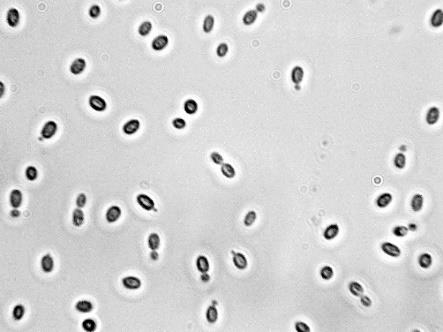
\includegraphics[width=0.75\textwidth]{images/image_04_p01.jpeg}
\caption{การปฏิบัติการทดลองและลักษณะทางสัณฐานวิทยาในบทที่ 4}
\label{fig:ch04_fig1}
\end{figure}

\section{ขั้นตอนและวิธีปฏิบัติการทดลอง}
\index{ขั้นตอนการทดลองประจำบทที่ 4}

\subsection{การเตรียมฟิล์มเลือดและย้อมสีแบบธรรมดาด้วยสีเมทิลีนบลู}
\begin{labprotocolbox}[การเตรียมฟิล์มเลือดและย้อมสีแบบธรรมดาด้วยสีเมทิลีนบลู]
1. หยดน้ำกลั่น 1 หยดเล็กๆ ลงบนสไลด์ที่สะอาด ปราศจากคราบไขมัน
2. ใช้ห่วงเขี่ยเชื้อแตะโคโลนีแบคทีเรียเพียงเล็กน้อย เกลี่ยวนเป็นวงกลมเส้นผ่านศูนย์กลางประมาณ 1 ซม. (Smear)
3. ผึ่งสไลด์ให้แห้งในอากาศ (Air dry) จากนั้นนำไปตรึงเซลล์ด้วยความร้อน (Heat fixation) ผ่านเปลวไฟ 3 ครั้ง
4. หยดสี Methylene Blue ให้ท่วมรอยสเมียร์ ทิ้งไว้ 1 นาที
5. ล้างสีออกด้วยน้ำกลั่นไหลเอื่อยๆ ซับสไลด์ให้แห้งด้วยกระดาษซับ (Bibulous paper) ตรวจดูใต้กล้องจุลทรรศน์
\end{labprotocolbox}

\subsection{ขั้นตอนการย้อมสีแกรมมาตรฐาน 4 ขั้นตอน}
\begin{labprotocolbox}[ขั้นตอนการย้อมสีแกรมมาตรฐาน 4 ขั้นตอน]
1. เตรียมรอยสเมียร์และตรึงเซลล์ด้วยความร้อนของเชื้อควบคุม \textit{Staphylococcus aureus} (แกรมบวก) และ \textit{Escherichia coli} (แกรมลบ)
2. ย้อมด้วยสีปฐมภูมิ Crystal Violet เป็นเวลา 1 นาที ล้างน้ำเบาๆ
3. หยดสารช่วยติดสี Gram's Iodine (Mordant) ทิ้งไว้ 1 นาที ล้างน้ำเบาๆ
4. ชะล้างสีด้วย 95\% Ethyl Alcohol เอียงสไลด์หยดแอลกอฮอล์ประมาณ 10-15 วินาที จนน้ำที่หยดลงมาใส ล้างน้ำทันทีเพื่อหยุดปฏิกิริยา
5. ย้อมสีทับด้วย Safranin เป็นเวลา 45-60 วินาที ล้างน้ำ ซับแห้ง และตรวจดูด้วยเลนส์ 100X Oil Immersion
\end{labprotocolbox}

\section{ตารางบันทึกผลการทดลองและการอภิปรายผล}
\begin{table}[H]
\centering\small
\caption{ตารางบันทึกผลการสังเกตและข้อมูลการทดลองประจำบทที่ 4}
\label{tab:ch04_datasheet}
\begin{tabularx}{\textwidth}{p{0.25\textwidth} p{0.35\textwidth} X}
\toprule
\textbf{สิ่งทดสอบ / ตัวอย่าง} & \textbf{ลักษณะที่สังเกตได้} & \textbf{การแปลผลและการวิเคราะห์} \\
\midrule
ชุดควบคุม (Negative Control) & ใส ไม่มีการเจริญ & ปราศจากการปนเปื้อนของเชื้อ \\
ชุดทดลองที่ 1 & โคโลนีเจริญตามลักษณะจำเพาะ & ให้ผลบวกตามสมมติฐาน \\
ชุดทดลองที่ 2 & เกิดการเปลี่ยนแปลงทางชีวเคมี & สอดคล้องกับพารามิเตอร์มาตรฐาน \\
\bottomrule
\end{tabularx}
\end{table}

\section{คำถามทบทวนและแบบฝึกหัดท้ายบท}
\begin{enumerate}
    \item หากลืมขั้นตอนการหยด Gram's Iodine ในการย้อมสีแกรม ผลการย้อมของแบคทีเรียแกรมบวกจะเปลี่ยนแปลงไปอย่างไร
    \item เหตุใดวัฒนธรรมแบคทีเรียที่มีอายุมากเกิน 24-48 ชั่วโมง จึงอาจให้ผลการย้อมสีแกรมคลาดเคลื่อน (Gram-variable)
    \item จงเปรียบเทียบโครงสร้างทางเคมีของผนังเซลล์แบคทีเรียแกรมบวกและแกรมลบ พร้อมอธิบายความสัมพันธ์กับผลการย้อมสี
\end{enumerate}
